\section{Summary of Key Findings}
\label{sec:summary}

Before detailing our experimental journey, we present the primary conclusions of this study. After a comprehensive evaluation across a range of methods, three distinct dynamical systems, and a wide range of noise levels, a clear verdict emerges. Performance was analyzed in two regimes: a "low-noise" regime ($\le 0.1\%$ noise) where precision is paramount, and a "high-noise" regime (1-2\% noise) where robustness is key.

The table below summarizes the performance of contender methods that demonstrated full data coverage for derivative orders 0 through 5. Methods are sorted by their overall average rank, giving equal weight to performance in both low- and high-noise regimes. Averages are calculated over orders 0-5.

% AUTO-GENERATED by gemini-analysis/generate_exploratory_tables.py
% To regenerate: ./scripts/04_generate_tables.sh
% Alternative versions (orders 3, 7) available as tab_summary_order{3,7}.tex
\input{../build/tables/publication/tab_summary_order5.tex}

\textbf{Our principal findings are as follows:}

\begin{enumerate}
    \item \textbf{Gaussian Process Regression (GPR) is the most robust and accurate method overall.} The Julia GPR implementation (\texttt{GP-Julia-AD}) and the improved Python variants (\texttt{GP-RBF-*}) are the clear winners, consistently occupying the top ranks in both low and high-noise regimes.
    \item \textbf{The optimal method depends on the noise level and derivative order.} While GPR is the best all-arounder, splines like \texttt{Dierckx-5} offer excellent precision in low-noise environments, making them a top choice for cleaner data. In the high-noise regime, the filtering-based \texttt{Savitzky-Golay} provides a computationally cheap and highly effective alternative, ranking solidly in the top half of contenders.
    \item \textbf{Theoretical limits matter.} Many common low-degree spline methods are, by definition, incapable of representing high-order derivatives, limiting their applicability.
\end{enumerate}

The subsequent sections of this paper will detail the experimental journey and analysis that led to these conclusions, providing a narrative account of our investigation and offering a practical framework for method selection.

\subsection{Visual Confirmation of Findings}

The quantitative results in the summary table are powerfully illustrated by a few key visualizations.

\begin{figure}[htbp]
\centering
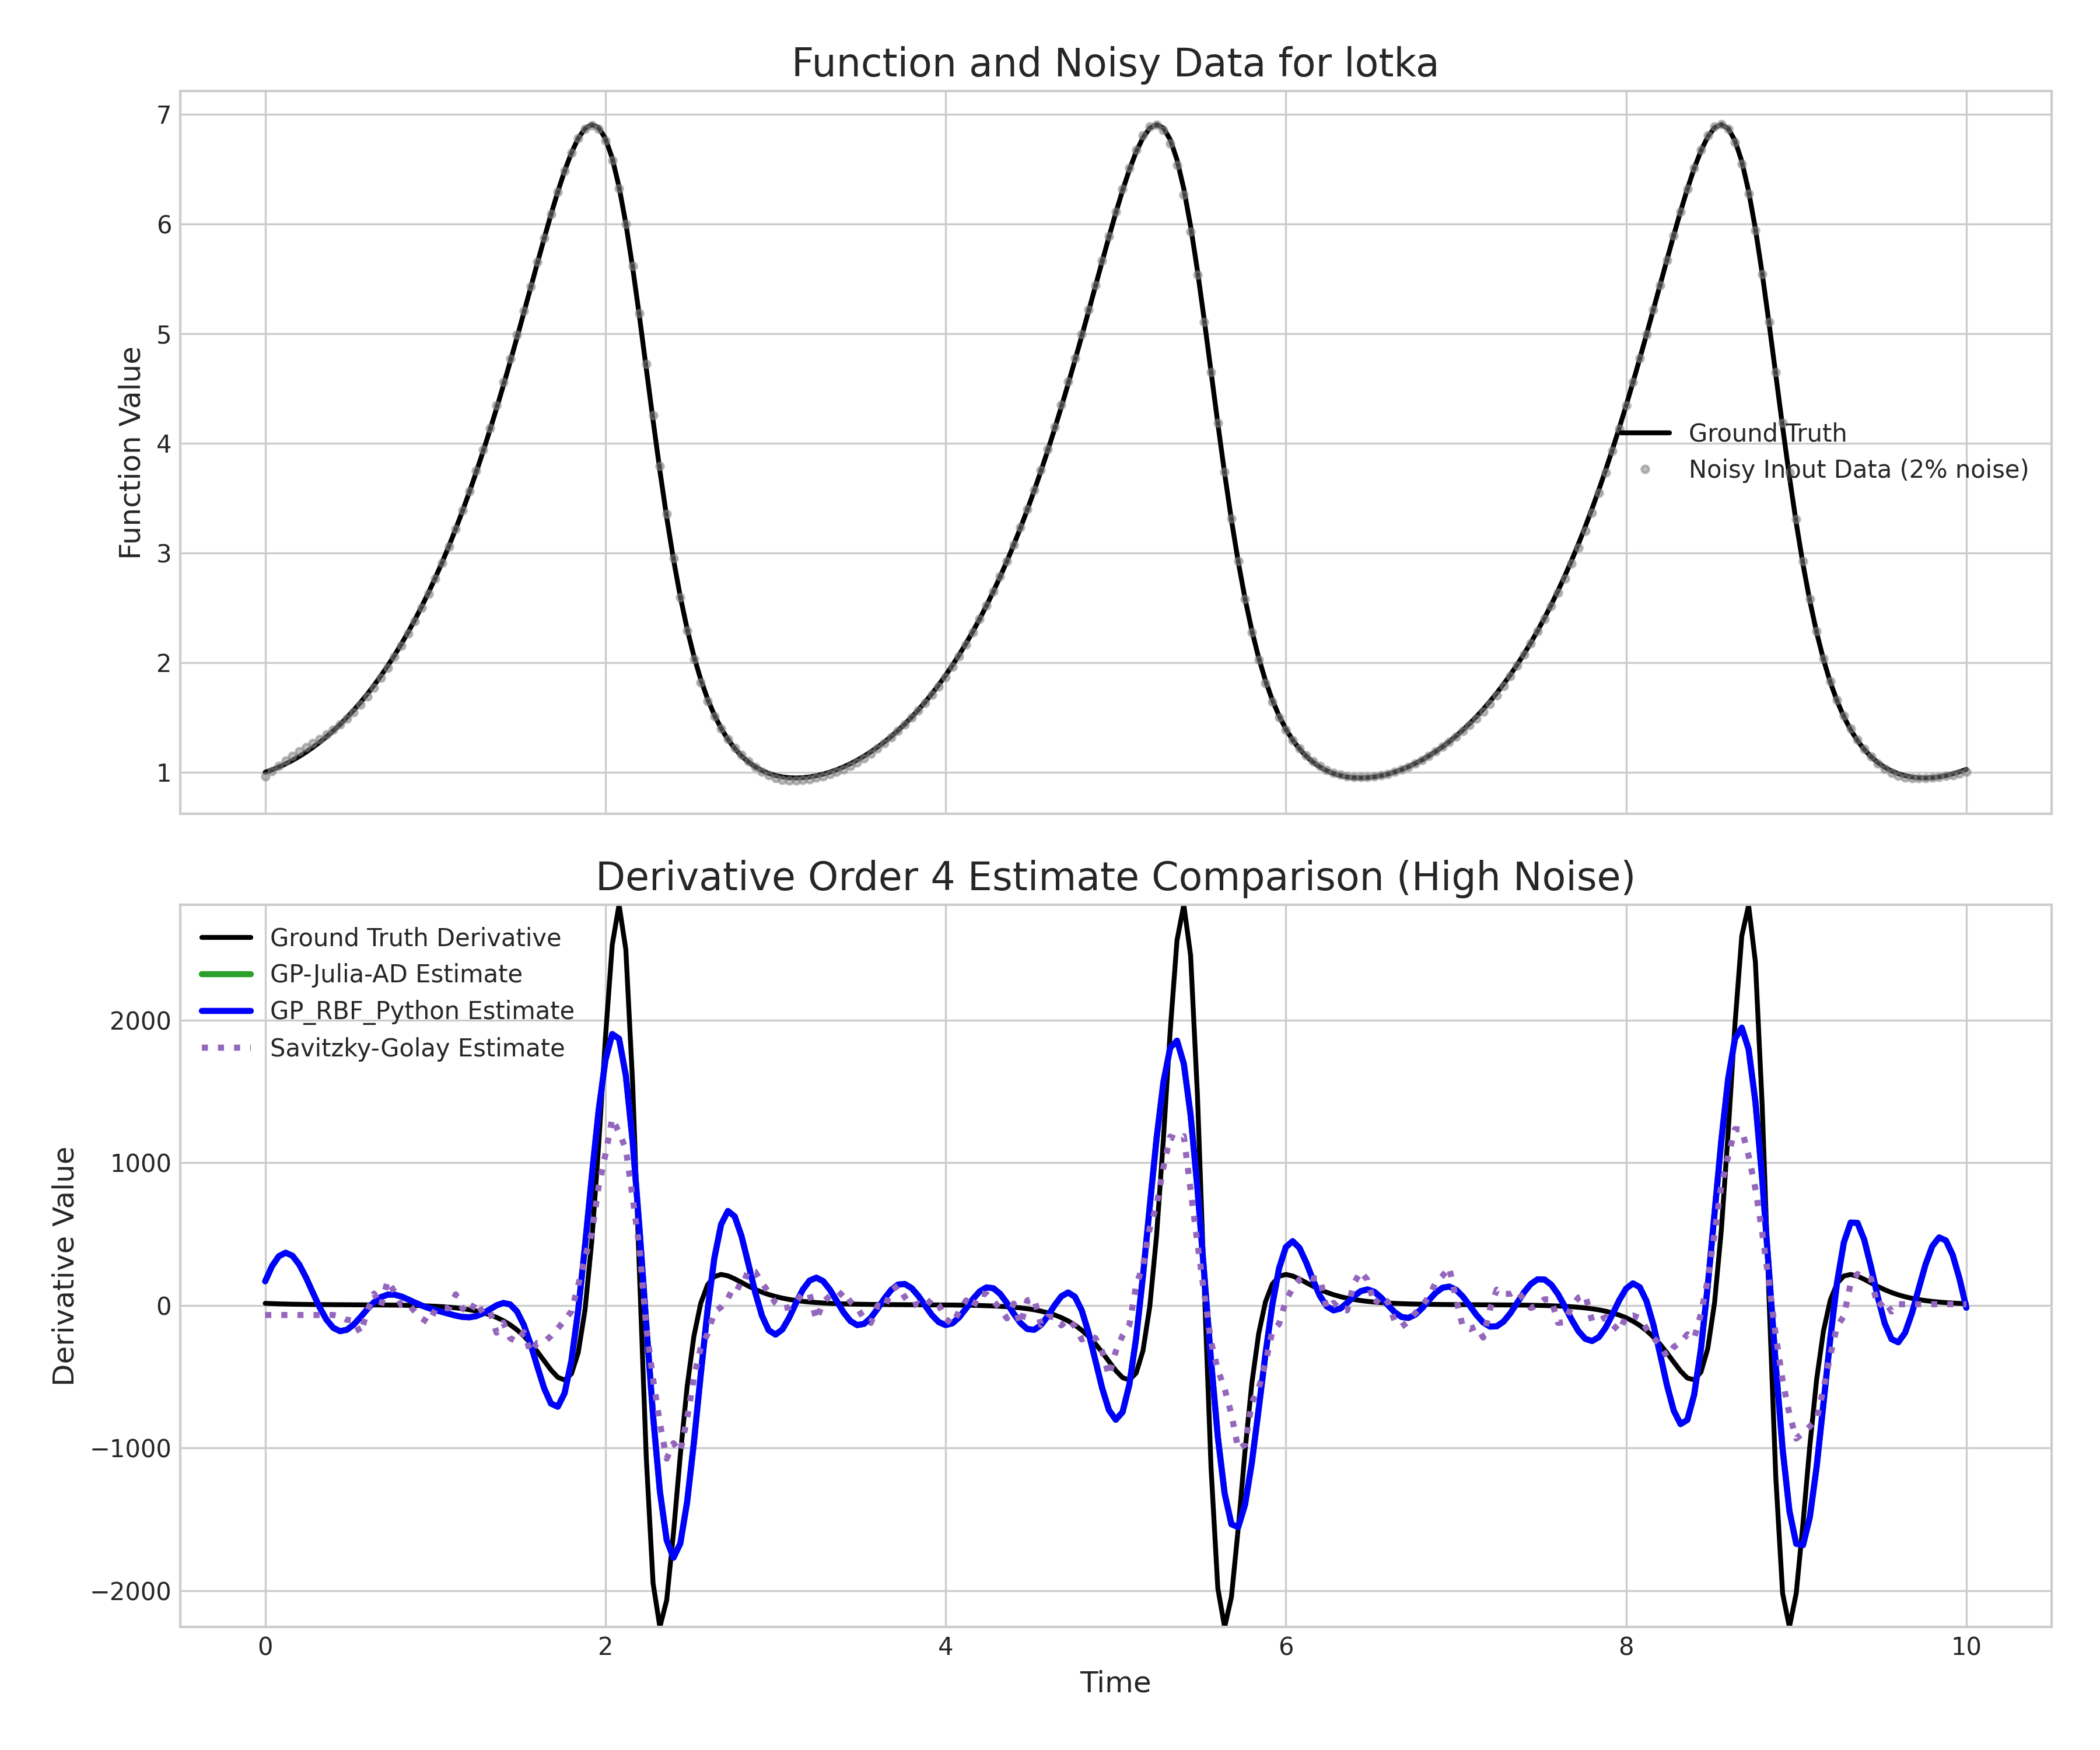
\includegraphics[width=0.9\textwidth]{high_noise_fit_comparison.png}
\caption{\textbf{High-Noise Performance (2\% noise, 4th derivative).} Three-panel comparison showing: (top) noisy input data as black points against gray ground truth, emphasizing the challenging signal-to-noise environment; (middle) derivative estimates from four methods representing different algorithmic approaches; (bottom) estimation errors revealing where each method succeeds or fails. \texttt{Fourier-GCV} achieves the lowest RMS error (306), followed by \texttt{GP-Julia-AD} (344), while \texttt{Savitzky-Golay} (457) and \texttt{Dierckx-5} (574) show progressively larger deviations. The error panel reveals that all methods struggle at the trajectory boundaries.}
\label{fig:high_noise_comp}
\end{figure}

\begin{figure}[htbp]
\centering
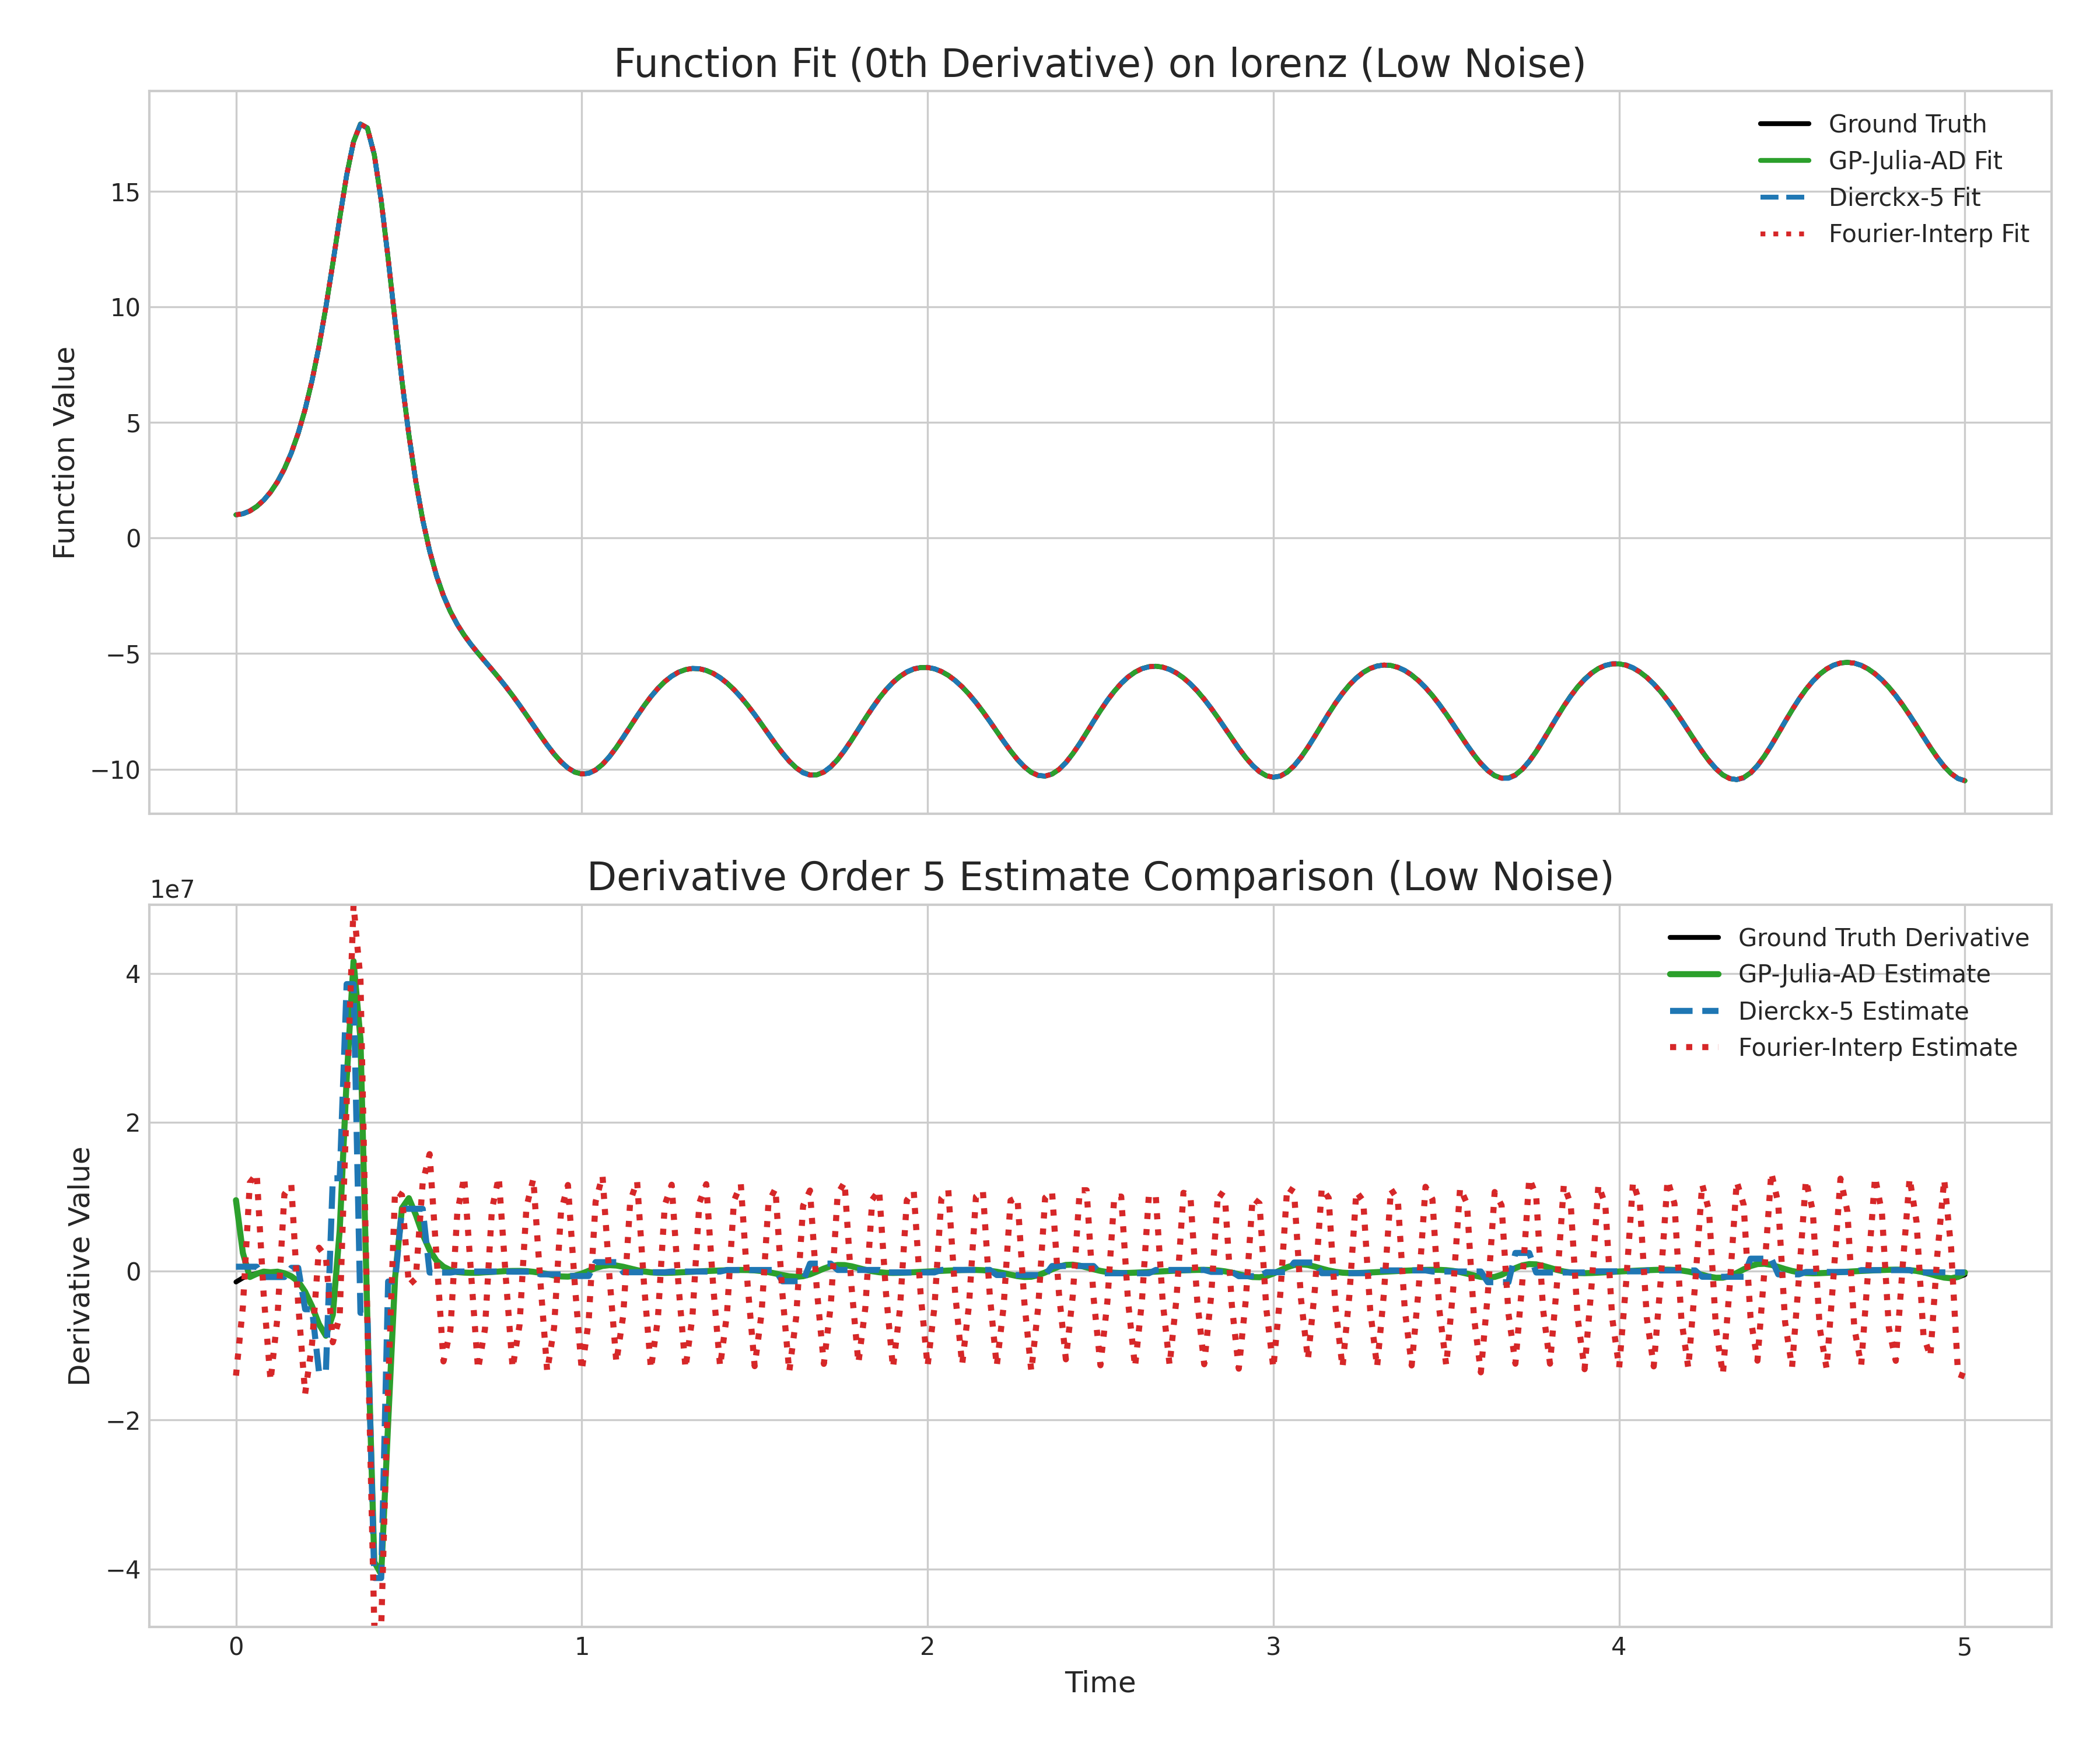
\includegraphics[width=0.9\textwidth]{low_noise_fit_comparison.png}
\caption{\textbf{Low-Noise Precision (1e-6 noise, 5th derivative).} Three-panel comparison in a low-noise regime: (top) noisy data points (black) are nearly imperceptible against gray ground truth; (middle) 5th-order derivative estimates from the top three methods; (bottom) estimation errors showing clear performance hierarchy. \texttt{GP-Julia-AD} dominates with RMS error of 272k, while \texttt{Dierckx-5} (3.1M) and \texttt{Fourier-GCV} (5.8M) show substantially larger errors. Even in this clean environment, high-order differentiation remains extremely challenging, with \texttt{GP-Julia-AD} achieving more than 10× better accuracy than competing methods.}
\label{fig:low_noise_comp}
\end{figure}

\begin{figure}[htbp]
\centering
\includegraphics[width=0.9\textwidth]{top_methods_heatmap.png}
\caption{\textbf{Performance Degradation with Increasing Derivative Order.} This heatmap shows the mean nRMSE for top methods at a 1\% noise level. The vertical axis is sorted by average performance across all orders. This visualization clearly shows that \texttt{GP-Julia-AD} maintains low error across all derivative orders, while other methods like \texttt{Dierckx-5} and \texttt{GSS} are highly accurate for low orders but degrade significantly as the order increases.}
\label{fig:heatmap}
\end{figure}

% Computational efficiency considerations are discussed in Section~\ref{sec:efficiency} rather than as a primary finding, due to implementation-dependent variability in timing measurements.
